\pdfoutput=1
\documentclass[11pt,a4paper]{article}
\usepackage{abhijit-research}
\renewcommand{\PaperCode}{P02}
\renewcommand{\PaperKind}{RESEARCH PAPER}
\renewcommand{\PaperVersion}{VERSION 1.0}
\renewcommand{\PaperDate}{AUGUST 2026}
\renewcommand{\PaperTitle}{Sequential Quantum Instruments}
\renewcommand{\PaperSubtitle}{Depletion, Regeneration, and Minimal Predictive State}
\renewcommand{\PaperFullTitle}{Sequential Quantum Instruments: Depletion, Regeneration, and Minimal Predictive State}
\renewcommand{\PaperShortTitle}{Sequential Quantum Instruments}
\renewcommand{\PaperKeywords}{quantum instrument; sequential measurement; Bell nonlocality; contextuality; predictive state; entropy rate}
\renewcommand{\PaperClassification}{Analytic theorems retain their displayed protocol assumptions. Processed-matrix results are exact for the supplied matrices and positivity completion. No result is generalized to all measurement systems.}
\renewcommand{\PaperCitation}{Singh, Abhijit. 2026. \textit{Sequential Quantum Instruments: Depletion, Regeneration, and Minimal Predictive State}. Research manuscript, version 1.0.}
\begin{document}
\MakeResearchTitle
\MakeResearchContents
\MakeResearchAbstract{%
Sequential measurement is analysed through the complete instrument object: an outcome map and its conditional successor state. A sharp alternating walk on one singlet is solved exactly, proving that the first local result destroys the reusable Bell resource while later conditional entropy remains positive. Repeated unread projective channels are classified by their fixed operator algebra, yielding the exact stationary witness value $m/d$ and the sharp rank-over-dimension compatibility floor. A Poisson equation gives the finite-time passage potential and the exact criterion for sustained contextual witnesses; the Yu-Oh no-reset protocol and KCBS selective-replacement thresholds are derived. A processed four-outcome Bell instrument is then physically completed and iterated in a common basis. Its current mark is the unique minimal predictive state, with exact stationary, spectral, information, and record-cost values.
}
\section{Operational object}
A measurement operation is represented by a quantum instrument, not by a probability distribution alone. The instrument produces both an outcome and a conditional successor state. The same distinction is required when a sequence is reused: outcome uncertainty, state memory, nonclassical certification, and physical record cost are separate quantities.

For a completely positive instrument $\{\mathcal I_a\}_a$,
\begin{equation}
p(a\mid\rho)=\Tr\mathcal I_a(\rho),\qquad
\rho'_a=\frac{\mathcal I_a(\rho)}{p(a\mid\rho)}.
\end{equation}
The unread channel is $\mathcal T=\sum_a\mathcal I_a$. All repeated-use calculations below preserve this complete object.

\part{Sharp sequential measurement of one singlet}
\section{Even-cycle protocol}
Let $n\ge4$ be even, $\delta=\pi/n$, $c=\cos\delta$, and $d=\cos(2\delta)$. Define
\begin{equation}
O(\theta)=\cos\theta\,\sigma_z+\sin\theta\,\sigma_x,
\end{equation}
and start from the singlet
\begin{equation}
|\Psi^-\rangle=\frac{|01\rangle-|10\rangle}{\sqrt2}.
\end{equation}
At global step $k$, measure $O(k\delta)$ on Alice for even $k$ and Bob for odd $k$, recording $X_k\in\{-1,+1\}$. Adjacent measurements act on different subsystems and are compatible; every measurement is rank-one and projective.

\begin{theorem}[Sharp-mark depletion]
Conditional on $X_0=a$, the post-measurement joint state is
\begin{equation}
\rho_{AB}^{(a)}=|a;0\rangle\langle a;0|_A\otimes|-a;0\rangle\langle-a;0|_B.
\end{equation}
Its entanglement negativity is zero. Every later selected local projective outcome keeps the state product. The same pair cannot generate a later Bell violation unless a new entangling operation is applied.
\end{theorem}
\begin{proof}
The singlet is perfectly anticorrelated in every common basis:
$(P_a(0)\otimes I)|\Psi^-\rangle\propto|a;0\rangle_A\otimes|-a;0\rangle_B$. This vector has Schmidt rank one. A local rank-one projector maps a product vector to another product vector or zero, so induction covers the remaining selected outcomes. The unread first measurement is a convex mixture of product states and is separable.
\end{proof}

\section{Exact entropy profile}
The first result is uniform. Singlet anticorrelation and the local two-step update give
\begin{align}
\Pr(X_1=b\mid X_0=a)&=\frac{1-abc}{2},\\
\Pr(X_k=x\mid X_{<k})&=\Pr(X_k=x\mid X_{k-2}=y)=\frac{1+xyd}{2},\qquad k\ge2.
\end{align}
With binary entropy $h_2$,
\begin{theorem}[Entropy profile]
\begin{align}
H(X_0)&=1,\\
H(X_1\mid X_0)&=h_2\!\left(\sin^2\frac{\pi}{2n}\right),\\
H(X_k\mid X_{<k})&=h_2\!\left(\cos^2\frac{\pi}{n}\right),\qquad k\ge2.
\end{align}
The trusted-model guessing probability after the seed is $\cos^2(\pi/n)$ and the conditional min-entropy is $-\log_2\cos^2(\pi/n)>0$.
\end{theorem}

\begin{table}[H]
\centering
\caption{Exact entropy values for representative even cycles.}
\begin{tabular}{cccc}
\toprule
$n$ & $1+H(X_1\mid X_0)$ & steady Shannon rate & steady guessing probability\\
\midrule
4 & 1.6009 & 1.0000 & 0.5000\\
6 & 1.3546 & 0.8113 & 0.7500\\
8 & 1.2333 & 0.6009 & 0.8536\\
\bottomrule
\end{tabular}
\end{table}

\begin{figure}[H]\centering
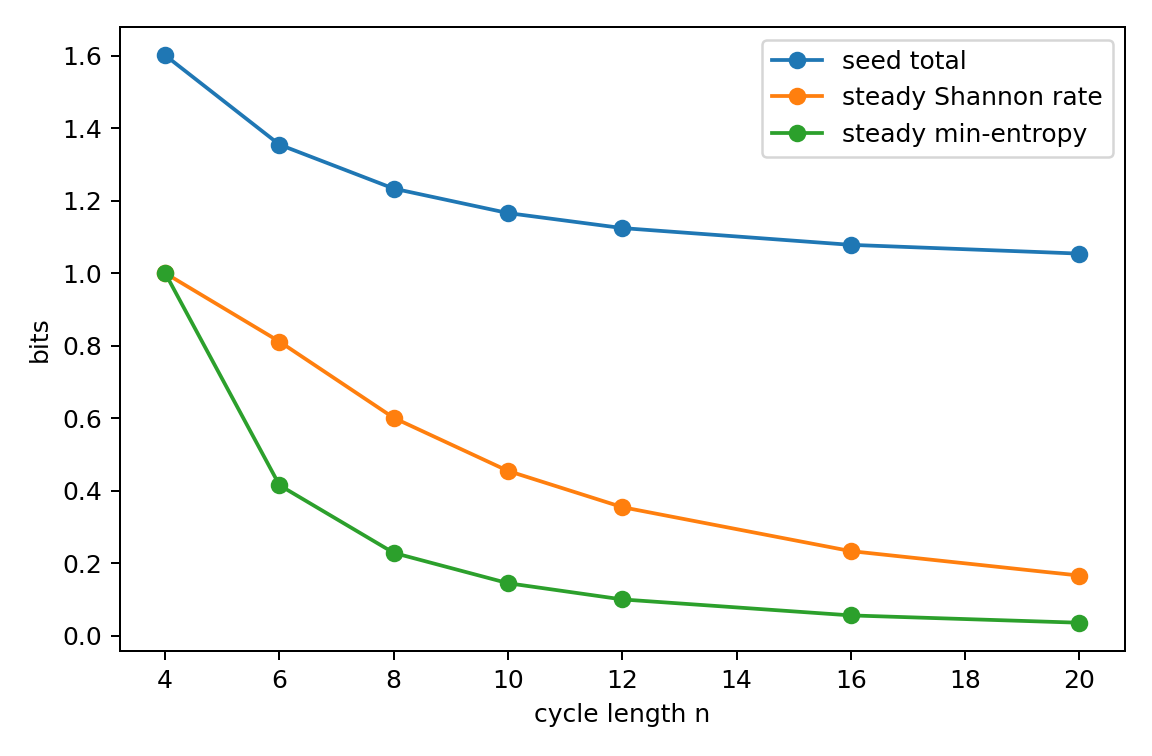
\includegraphics[width=.72\linewidth]{figures/p2_entropy_profile.png}
\caption{Seed entropy, steady Shannon rate, and trusted-model min-entropy.}
\end{figure}

\section{Geometric correlator depletion}
Define $R_k=\mathbb E[X_kX_{k+1}]$. Since $\mathbb E[X_{k+2}\mid X_k]=dX_k$,
\begin{theorem}[Geometric decay]
\begin{equation}
\boxed{R_k=-\cos\frac{\pi}{n}\,\cos^k\frac{2\pi}{n}.}
\end{equation}
For $n=4$, all correlators after $R_0$ vanish exactly. The signed sum over every later $n$-step block tends to zero.
\end{theorem}
A fresh-singlet experiment on every edge instead gives the chained magnitude $n\cos(\pi/n)$. These are different resource schedules, not two readings of the same sequential resource.

\begin{figure}[H]\centering
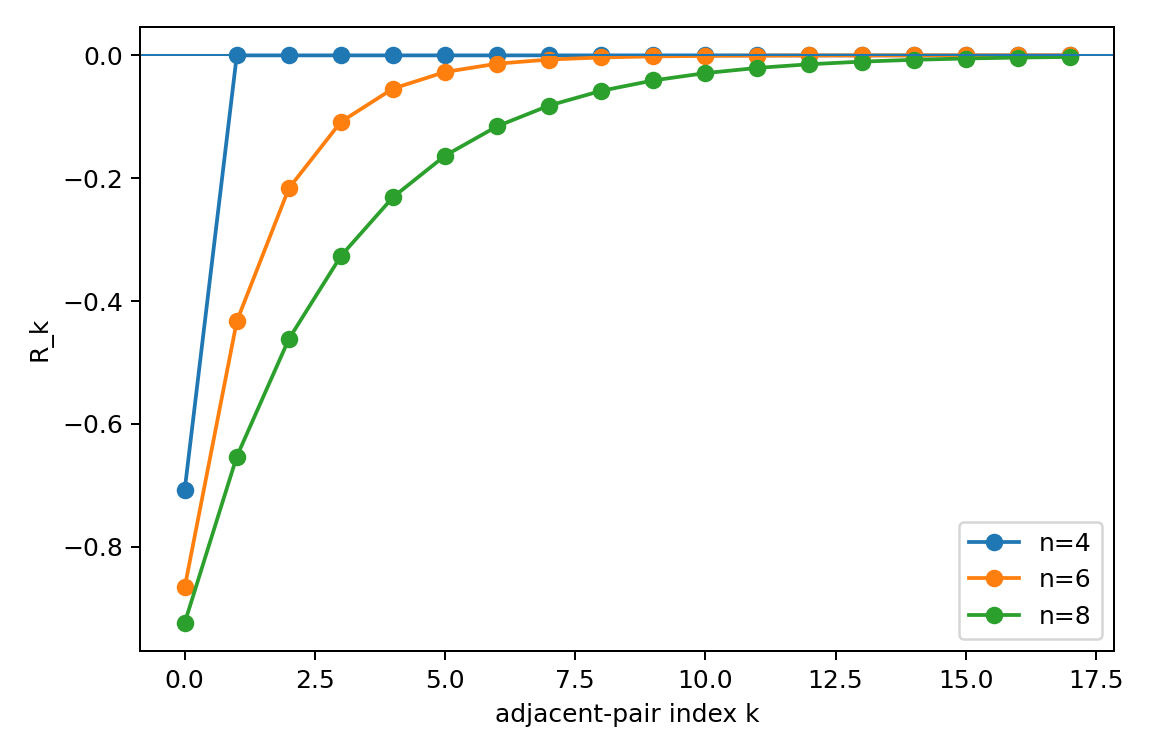
\includegraphics[width=.72\linewidth]{figures/p2_correlator_decay.png}
\caption{Exact adjacent-correlator decay for three even cycles.}
\end{figure}

\begin{theorem}[Certificate separation]
Positive post-seed conditional entropy does not imply a post-seed Bell-device-independent certificate from the same walked pair.
\end{theorem}
\begin{proof}
After the first result the conditional joint state is product. The remaining process has a local causal realization: sample the correlated seed pair, then update the two sides with independent local transition coins. The later statistics therefore do not require a nonlocal resource, while the Shannon and trusted-model min-entropies remain positive.
\end{proof}

\part{Repeated contextual instruments}
\section{Unital self-idling}
For a projector $P$, the unread Lueder channel
\begin{equation}
\mathcal D_P(X)=PXP+(I-P)X(I-P)
\end{equation}
is an orthogonal projection in Hilbert-Schmidt operator space. For a periodic sequence $P_0,\ldots,P_{m-1}$, let $\mathcal T=\mathcal D_{P_{m-1}}\cdots\mathcal D_{P_0}$.

\begin{theorem}[Unital self-idling]
The fixed operator space is the intersection of the commutants of the $P_j$. If the family is irreducible, $\mathcal T^k(\rho)\to I/d$ for every initial state. An unweighted rank-one witness therefore idles at
\begin{equation}
\boxed{W_{\rm idle}=m/d.}
\end{equation}
\end{theorem}
This explains the exact values $5/3$, $7/5$, and $2$ in the audited walks. Comparing $m/d$ with the noncontextual bound $\alpha(G)$ gives strict idling, facet idling, or state-independent violation.

\begin{theorem}[Adjacent-orthogonality floor]
If $P_jP_{j+1}=0$ and the stationary state is $I/d$, the asymptotic fraction of forced next steps obeys
\begin{equation}
\tau\ge\frac1m\sum_j\frac{\rank P_j}{d}.
\end{equation}
For rank-one tests the sharp floor is $1/d$. The frequently observed value $1/3$ is the qutrit instance, not a universal constant.
\end{theorem}

\section{Passage potential and stationary engine criterion}
For randomized contexts $c$ and score $g(c,x)$, define the averaged reward operator $R$ and unread channel $\mathcal T$. If $\mathcal T$ is primitive with stationary state $\sigma$, put $q=\Tr(\sigma R)$.
\begin{theorem}[Poisson passage potential]
There is a Hermitian $K$, unique up to a scalar, satisfying
\begin{equation}
K-\mathcal T^*(K)=R-qI.
\end{equation}
For the mean evolution,
\begin{equation}
\sum_{t=0}^{N-1}\Tr(\rho_tR)=Nq+\Tr(\rho_0K)-\Tr(\rho_NK).
\end{equation}
The long-run witness exceeds the noncontextual bound exactly when $q>\beta_{\rm NC}$.
\end{theorem}
If $R=qI$, then $K=0$ and the expected witness is $q$ at every round for every state; no return to a preferred state is required.

\section{Yu-Oh and KCBS calculations}
For the 13-ray Yu-Oh construction,
\begin{equation}
L_{YO}=\frac{25}{3}I,
\end{equation}
while the noncontextual bound is $8$. With the displayed singleton/edge randomization, the quantum mean is $1/3$, the noncontextual mean is at most $8/25$, and the per-round gap is $1/75$.

For the five-ray KCBS family, replacement after a no outcome is optimal within the audited outcome-selective family. The exact thresholds are
\begin{align}
r_{\rm no}^*&=0.8396425434,\\
c_{\min}&=0.5037855260,\\
r_{\rm uniform}^*&=0.5115311845.
\end{align}
Replacement after yes outcomes alone reaches only $1.9098300563<2$.

\part{A complete four-outcome marked instrument}
\section{Physical completion and common basis}
Let
\begin{equation}
E_a=\sum_re_{ar}|v_{ar}\rangle\langle v_{ar}|,\qquad
\sigma_a=\sum_sq_{as}|w_{as}\rangle\langle w_{as}|.
\end{equation}
The Kraus family
\begin{equation}
K_{asr}=\sqrt{e_{ar}q_{as}}\,|w_{as}\rangle\langle v_{ar}|
\end{equation}
realizes $\mathcal I_a(\rho)=\Tr(E_a\rho)\sigma_a$. The processed realization contains 60 nonzero Kraus operators. The complete classical-quantum Choi operator is
\begin{equation}
\mathbb J=\sum_a|a\rangle\langle a|_C\otimes\sigma_a\otimes E_a^{\mathsf T}.
\end{equation}
One nonpositive tomography estimate is repaired by retaining Bell-basis populations and scaling coherences by the maximal positivity factor
\begin{equation}
\eta_*=0.708418699729814.
\end{equation}
Effects and conditional states must be transformed into one common basis before repeated-use multiplication. Omitting this transformation changes the transition law by Frobenius norm $0.541915971853$.

\section{Corrected transition law and minimal predictive state}
The corrected column-stochastic law is
\begin{equation}
C=\begin{pmatrix}
0.43696297&0.19810609&0.20644079&0.14060033\\
0.16017410&0.46165671&0.13951861&0.22362294\\
0.24443666&0.11892971&0.46061556&0.17659060\\
0.15842628&0.22130750&0.19342504&0.45918613
\end{pmatrix}.
\end{equation}
Every pair of columns has positive total-variation distance, so no two marks can be merged in a first-order predictive state.

\begin{theorem}[Minimal mark state]
The four current marks are the unique coarsest predictive states for all later repeated uses of the processed instrument.
\end{theorem}

The stationary law and nontrivial eigenvalues are
\begin{equation}
\pi=(0.24327934,0.24563854,0.24991431,0.26116781),
\end{equation}
\begin{equation}
\spec(C)=\{1,0.35301358,0.27498875,0.19041902\}.
\end{equation}
Writing $\Pi=\pi\mathbf1^{\mathsf T}$ and $R=C-\Pi$ gives $C^n=\Pi+R^n$.

\section{Information loss and continuing entropy}
For a uniform initial source label $J$,
\begin{align}
I(J;A_0)&=0.4720622220\ \text{bits},\\
I(J;A_1)&=0.0409311197\ \text{bits}.
\end{align}
Only $8.6707\%$ remains after one reuse. At stationarity,
\begin{align}
H(A_t)&=1.9994586368\ \text{bits},\\
h=H(A_{t+1}\mid A_t)&=1.8413629168\ \text{bits/use},\\
I(A_t;A_{t+1})&=0.1580957201\ \text{bits}.
\end{align}
The best next-mark probability is $0.4547437955$, giving conditional min-entropy $1.1368741409$ bits.

For surprisal, the centred Poisson potential is
\begin{equation}
k=(0.03023948,-0.02314357,0.00046185,-0.00684276),
\end{equation}
and the finite-time mean error is at most $0.06047896/N$ bits per use.

\section{Record cost}
With the previous mark available as side information, optimal cyclic compression and erasure obey
\begin{equation}
Q_{\min}\ge k_BT\ln2\,h=1.2763355141\,k_BT
\end{equation}
per use. Avoiding reset requires memory growth at $1.8413629168$ bits per use.

\section{Scope and exact claim boundary}
The singlet and contextuality theorems apply to their displayed protocols. The four-outcome results are exact for the processed public matrices and the displayed positive completion. No universal claim about all sequential measurements follows. Raw conditional entropy, trusted-model min-entropy, nonclassical witness value, source memory, and physical record cost remain separate ledger entries.

\appendix
\section{Reproducibility table}
\begin{longtable}{p{.34\linewidth}p{.56\linewidth}}
\toprule
Object & Check\\\midrule
Even-cycle depletion & product state after first result; negativity $1/2\to0$\\
Entropy & exact $n=4,6,8$ values and positive post-seed min-entropy\\
Correlator & $R_k=-c d^k$ and geometric block extinction\\
Unital cycles & fixed commutant, $m/d$ idling, rank/$d$ floor\\
Contextual regeneration & Yu-Oh operator identity and KCBS thresholds\\
Marked instrument & positivity repair, Kraus completeness, Choi positivity, basis conversion, stationarity, information decay, Poisson potential\\
\bottomrule
\end{longtable}


\section{Full depletion and certificate proofs}
Let $P_a(\theta)=(I+aO(\theta))/2$. The singlet satisfies perfect anticorrelation in every common basis:
\begin{equation}
(P_a(0)\otimes I)|\Psi^-\rangle
\propto |a;0\rangle_A\otimes|-a;0\rangle_B.
\end{equation}
This selected state has Schmidt rank one and zero negativity. The unread first result is the convex mixture of the two selected product states and is separable. Every later selected local rank-one projector preserves product form. Thus the first sharp record, not the second, consumes the same pair's future Bell resource.

Singlet anticorrelation gives
\begin{equation}
\Pr(X_1=b\mid X_0=a)=\frac{1-ab\cos(\pi/n)}2,
\end{equation}
and for $k\ge2$ the most recent result on the same side is sufficient:
\begin{equation}
\Pr(X_k=x\mid X_{<k})=
\frac{1+xX_{k-2}\cos(2\pi/n)}2.
\end{equation}
Hence
\begin{align}
H(X_0)&=1,\\
H(X_1\mid X_0)&=h_2\!\left(\sin^2\frac{\pi}{2n}\right),\\
H(X_k\mid X_{<k})&=h_2\!\left(\cos^2\frac{\pi}{n}\right),\qquad k\ge2.
\end{align}
The trusted-model guessing probability is $\cos^2(\pi/n)$ and the conditional min-entropy is its negative base-two logarithm.

The adjacent correlator obeys
\begin{equation}
R_{k+1}=\cos(2\pi/n)R_k,
\qquad R_0=-\cos(\pi/n),
\end{equation}
therefore
\begin{equation}
R_k=-\cos\frac{\pi}{n}\cos^k\frac{2\pi}{n}.
\end{equation}
For $n=4$, every correlator after the first vanishes exactly. A fresh-pair chained experiment instead supplies a new singlet at every edge and gives $n\cos(\pi/n)$. Those are different resource schedules, not two measurements of one conserved violation.

\begin{table}[H]\centering
\caption{Exact entropy profile of the sharp even-cycle walk.}
\begin{tabular}{cccc}
\toprule
$n$&seed $1+H(X_1\mid X_0)$&steady rate&guess probability\\\midrule
4&1.6009&1.0000&0.5000\\
6&1.3546&0.8113&0.7500\\
8&1.2333&0.6009&0.8536\\
\bottomrule
\end{tabular}
\end{table}

\section{Complete stationary witness derivation}
For a sharp projector $P$, the unread channel
\begin{equation}
\mathcal D_P(X)=PXP+(I-P)X(I-P)
\end{equation}
is the Hilbert--Schmidt orthogonal projection onto the commutant of $P$. A product of such channels fixes exactly the intersection of the commutants. If the projectors are irreducible, only scalar operators survive and every state converges to $I/d$. For $m$ rank-one tests,
\begin{equation}
W_{\rm idle}=\sum_{j=1}^m\Tr\left(\frac{I}{d}P_j\right)=\frac md.
\end{equation}
If adjacent tests are orthogonal, every preceding yes result forces the next answer to be no. At stationarity the forced-step fraction satisfies
\begin{equation}
\tau\ge\frac1m\sum_j\frac{\rank P_j}{d},
\end{equation}
which becomes $1/d$ for rank-one tests. The earlier apparent one-third constant is therefore the qutrit instance.

For a repeated instrument with averaged channel $\mathcal T$, reward operator $R$, and stationary state $\sigma$, put $q=\Tr(\sigma R)$. On the centred subspace the Poisson equation
\begin{equation}
K-\mathcal T^*(K)=R-qI
\end{equation}
has a solution under primitivity, giving
\begin{equation}
\sum_{t=0}^{N-1}\Tr(\rho_tR)
=Nq+\Tr(\rho_0K)-\Tr(\rho_NK).
\end{equation}
Thus the long-run witness is determined by $q$, while $K$ is a bounded transient potential. If $R=qI$, the expected score is state-independent on every round and no reset is required.

\section{Exact contextual regeneration values}
For the 13-ray state-independent witness, direct projector multiplication gives the scalar operator used in the protocol and an exact per-round separation of $1/75$ from the noncontextual limit. For the five-ray family, symmetry reduces the stationary state to one target-overlap coordinate. Selective replacement after a no result is optimal within the audited family. The thresholds are
\begin{align}
r_{\rm no}^*&=0.8396425434,\\
c_{\min}&=0.5037855260,\\
r_{\rm uniform}^*&=0.5115311845,
\end{align}
and yes-only replacement reaches only $1.9098300563<2$.

\section{Corrected four-record instrument}
After expressing effects and returned states in one basis, the transition matrix is
\begin{equation}
C=\begin{pmatrix}
0.43696297&0.19810609&0.20644079&0.14060033\\
0.16017410&0.46165671&0.13951861&0.22362294\\
0.24443666&0.11892971&0.46061556&0.17659060\\
0.15842628&0.22130750&0.19342504&0.45918613
\end{pmatrix}.
\end{equation}
Its stationary law is
\begin{equation}
\pi=(0.24327934,0.24563854,0.24991431,0.26116781),
\end{equation}
and every pair of columns has positive total-variation distance, proving that the four current records are the unique coarsest first-order predictive states. The exact information ledger is
\begin{align}
H(A_{t+1})&=1.9994586368,\\
H(A_{t+1}\mid A_t)&=1.8413629168,\\
I(A_t;A_{t+1})&=0.1580957201
\end{align}
 bits. The finite-memory Landauer floor is therefore $1.2763355141\,k_BT$ per use when the previous record is retained as side information.

\begin{table}[H]\centering
\caption{Decay of retained source information in the corrected repeated instrument.}
\begin{tabular}{ccc}
\toprule
reuse $t$&$I(J;A_t)$ bits&optimal source-guess accuracy\\\midrule
0&0.4720622220&0.6232838703\\
1&0.0409311197&0.3514199523\\
2&0.0040117838&0.2790063220\\
3&0.0004285525&0.2586660216\\
4&$4.8954\times10^{-5}$&0.2526827310\\
10&$1.7447\times10^{-10}$&0.2500040417\\
\bottomrule
\end{tabular}
\end{table}

\section{Reproduction obligations}
A full reproduction verifies projector identities, selected and unread negativity, transition probabilities, entropies, correlator decay, fixed spaces, Poisson telescoping, contextual bounds, threshold optimization, basis transformation, physical positivity repair, Kraus completeness, Choi positivity, stationary law, and information decay. Public matrix calculations are exact for the supplied processed estimates; population uncertainty requires the raw-count covariance.

\begin{thebibliography}{99}
\bibitem{bell} J. S. Bell, On the Einstein Podolsky Rosen paradox, Physics 1 (1964), 195--200.
\bibitem{braunstein} S. L. Braunstein and C. M. Caves, Wringing out better Bell inequalities, Annals of Physics 202 (1990), 22--56.
\bibitem{pironio} S. Pironio et al., Random numbers certified by Bell's theorem, Nature 464 (2010), 1021--1024.
\bibitem{kcbs} A. A. Klyachko et al., Simple test for hidden variables in spin-1 systems, Physical Review Letters 101 (2008), 020403.
\bibitem{yuoh} S. Yu and C. H. Oh, State-independent proof of the Kochen--Specker theorem with 13 rays, Physical Review Letters 108 (2012), 030402.
\bibitem{leupold} F. M. Leupold et al., Sustained state-independent quantum contextual correlations from a single ion, Physical Review Letters 120 (2018), 180401.
\bibitem{kraus} K. Kraus, States, Effects, and Operations, Springer, 1983.
\bibitem{meyn} S. P. Meyn and R. L. Tweedie, Markov Chains and Stochastic Stability, Springer, 2009.
\bibitem{landauer} R. Landauer, Irreversibility and heat generation in the computing process, IBM Journal of Research and Development 5 (1961), 183--191.
\bibitem{reeb} D. Reeb and M. M. Wolf, An improved Landauer principle with finite-size corrections, New Journal of Physics 16 (2014), 103011.
\end{thebibliography}
\end{document}
